\documentclass[12pt,a4paper]{report}

% Packages
\usepackage[utf8]{inputenc}
\usepackage{amsmath, amssymb}
\usepackage{graphicx}
\usepackage{hyperref}
\usepackage{geometry}
\usepackage{fancyhdr}
\usepackage{titlesec}
\usepackage{setspace}
\usepackage{listings}
\usepackage{color}
\usepackage{natbib}
\usepackage{tocbibind}
\usepackage{float}
\usepackage{dirtytalk}
\usepackage{dsfont}
\usepackage{algorithm}
\usepackage{algorithmic}

% Geometry settings
\geometry{
    a4paper,
    left=30mm,
    right=25mm,
    top=25mm,
    bottom=25mm,
}

% Header and Footer
\fancyhf{}
\fancyhead[L]{\leftmark}
\fancyhead[R]{\thepage}
\setlength{\headheight}{15pt}
\pagestyle{fancy}

% Title formatting
\titleformat{\chapter}[hang]{\LARGE\bfseries}{\thechapter.}{2pc}{}
\titleformat{\section}[hang]{\large\bfseries}{\thesection.}{1pc}{}

% Code Listings settings
\definecolor{codegray}{rgb}{0.5,0.5,0.5}
\definecolor{codegreen}{rgb}{0,0.6,0}
\definecolor{codeblue}{rgb}{0,0,0.9}
\definecolor{backcolour}{rgb}{0.95,0.95,0.92}

\lstdefinestyle{mystyle}{
    backgroundcolor=\color{backcolour},
    commentstyle=\color{codegreen},
    keywordstyle=\color{codeblue},
    numberstyle=\tiny\color{codegray},
    stringstyle=\color{codeblue},
    basicstyle=\ttfamily\footnotesize,
    breakatwhitespace=false,
    breaklines=true,
    captionpos=b,
    keepspaces=true,
    numbers=left,
    numbersep=5pt,
    showspaces=false,
    showstringspaces=false,
    showtabs=false,
    tabsize=2
}

\lstset{style=mystyle}

\newenvironment{acknowledgements}
  {\cleardoublepage\thispagestyle{plain}\chapter*{Acknowledgements}}
  {\cleardoublepage}

% Prevent duplicate destination identifiers
\hypersetup{pageanchor=true}

% Document start
\begin{document}

% Title Page
\begin{titlepage}
    \begin{center}
        \vspace*{1cm}

        \Huge
        \textbf{Incorporating Deep Descriptive Clustering into the DECCS Algorithm}

        \vspace{0.5cm}
        \LARGE
        for Enhanced Interpretability and Performance on AwA and APY Datasets

        \vspace{1.5cm}

        \textbf{Mehdi Benabed}

        \vfill

        A thesis submitted in partial fulfillment\\
        of the requirements for the degree of\\
        Master of Science in Computer Science

        \vspace{0.8cm}

        \includegraphics[width=0.4\textwidth]{figs/Uni_Logo_2016.png}

        \Large
        Faculty of Computer Science\\
        University of Vienna\\
        Austria\\
        \today

    \end{center}
\end{titlepage}

% Abstract
\begin{abstract}
    \addcontentsline{toc}{chapter}{Abstract}
    This thesis introduces a novel approach to enhance the interpretability of the Deep Embedded Clustering with Consensus Representations (DECCS) algorithm by incorporating principles from the Deep Descriptive Clustering (DDC) framework. DECCS has shown significant advances in clustering precision but often falls short in terms of interpretability. This research aims to bridge this gap by refining the DECCS algorithm to not only generate clusters but also provide meaningful, cluster-level explanations that enhance transparency and comprehensibility in the clustering process.

The methodology involves adapting DECCS to effectively interface with specific datasets used in the DDC experimental framework, particularly the Animals with Attributes (AwA) and the aPascal \& aYahoo (aPY) datasets. This adaptation incorporates DDC’s symbolic level representations into DECCS, aiming to create a seamless integration between raw data clustering and semantic interpretability.

A significant aspect of this thesis is the integration of DDC’s interpretative capabilities with DECCS’s clustering method. This integration strives to maintain the high quality of cluster formation inherent to DECCS while elevating the level of interpretability. The dual focus ensures that the resulting predictions are both accurate and comprehensible, providing insights into the underlying structure and relationships within the data.

This thesis evaluates the integrated approach through extensive experiments, assessing both clustering performance and the quality of explanations generated. The evaluation includes comparisons with recent advancements and foundational algorithms in the field, demonstrating the efficacy of combining DECCS with DDC principles. By highlighting the advantages of this combination in practical clustering applications, the research contributes to the field of data clustering by offering a novel methodology that combines the efficiency of DECCS with the interpretative power of DDC.

Overall, this research sets a new benchmark for transparent, understandable, and insightful data analysis in various domains, addressing the increasing demand for interpretability and accountability in complex data clustering.
\end{abstract}

% Acknowledgements
%\begin{acknowledgements}
%    \addcontentsline{toc}{chapter}{Acknowledgements}
%    Write your acknowledgements here. Thank those who helped you with your research and thesis.
%\end{acknowledgements}

% Table of Contents
\tableofcontents
\listoffigures
\listoftables

% Chapters
\chapter{Introduction}
\section{Background}

The growing complexity of modern datasets necessitates a paradigm shift in algorithmic approaches, particularly in the realm of data clustering. Deep learning has revolutionized machine learning across many domains \citep{LeCun2015}, and its integration with clustering has opened new possibilities for unsupervised learning \citep{Ren2024}. While Deep Embedded Clustering with Consensus Representations (DECCS) has made significant strides in clustering precision, it highlights the critical limitation of interpretability within these advances. This limitation is becoming increasingly problematic in a landscape of data analysis that demands greater transparency and accountability \citep{Guidotti2018}. This research aims to address this gap by integrating the strengths of the Deep Descriptive Clustering (DDC) framework.

Interpretability in clustering is crucial for several reasons. In many real-world applications, such as healthcare, finance, and autonomous systems, the ability to understand and trust the decisions made by clustering algorithms can significantly impact decision-making processes. For instance, in healthcare, understanding why a group of patients has been clustered together can lead to better diagnoses and personalized treatments. Similarly, in finance, transparent clustering can help in risk assessment and fraud detection.

While DECCS excels in efficiently segmenting complex datasets, its opaque decision-making processes pose significant barriers in contexts where understanding the `why' behind data clusters is as crucial as the `what'. Integrating DDC principles is a preliminary step towards interpreting the clustering process, thus enhancing utility and transparency in data analysis \citep{Saisubramanian2020}.

Furthermore, the practical implications of this integration are profound. By focusing on a specific dataset---the Animals with Attributes 2 (AwA2)---this research moves beyond theoretical advancements to demonstrate how the DECCS algorithm can be adapted to incorporate semantic supervision, thereby exploring its potential utility for interpretable clustering tasks.

\section{Problem Statement}

\subsection{Formal Problem Definition}

Given a dataset $\mathcal{D} = \{(\mathbf{x}_i, \mathbf{t}_i)\}_{i=1}^{N}$ where $\mathbf{x}_i \in \mathbb{R}^D$ represents high-dimensional input data (e.g., images) and $\mathbf{t}_i \in [0,1]^T$ represents associated semantic attribute vectors, the goal is to learn:

\begin{enumerate}
    \item An encoder function $f_\theta: \mathbb{R}^D \rightarrow \mathbb{R}^d$ that maps inputs to a low-dimensional embedding space ($d \ll D$)
    \item A cluster assignment function $g: \mathbb{R}^d \rightarrow \{1, \ldots, K\}$ that partitions the embedded data into $K$ clusters
    \item An explanation function $h: \{1, \ldots, K\} \rightarrow 2^{\{1,\ldots,T\}}$ that associates each cluster with a subset of semantic attributes
\end{enumerate}

The optimization objectives are:

\begin{equation}
    \min_{\theta, g, h} \underbrace{\mathcal{L}_{recon}(\theta)}_{\text{reconstruction}} + \lambda_1 \underbrace{\mathcal{L}_{tag}(\theta)}_{\text{semantic alignment}} + \lambda_2 \underbrace{\mathcal{L}_{consensus}(\theta, g)}_{\text{ensemble agreement}}
\end{equation}

subject to the constraint that the explanations $h$ are:
\begin{itemize}
    \item \textbf{Concise}: Each cluster is described by a small number of attributes
    \item \textbf{Discriminative}: Attribute sets distinguish clusters from one another
    \item \textbf{Faithful}: Attributes accurately reflect the characteristics of cluster members
\end{itemize}

\subsection{Key Challenges}

This problem presents several technical challenges:

\begin{enumerate}
    \item \textbf{Multi-objective optimization}: Balancing reconstruction quality, semantic alignment, and clustering performance requires careful hyperparameter tuning and may involve trade-offs \citep{Ruder2017, Crawshaw2020}.

    \item \textbf{Scalability}: Computing consensus across multiple clustering algorithms on large datasets is computationally expensive.

    \item \textbf{Semantic gap}: Bridging the gap between low-level visual features and high-level semantic attributes requires learning representations that capture both \citep{Bengio2013}.

    \item \textbf{Evaluation complexity}: Assessing both clustering quality and explanation quality requires multiple complementary metrics.
\end{enumerate}

\section{Research Objectives}

The primary objectives of this research are as follows:

\begin{itemize}
    \item \textbf{Enhance Interpretability of DECCS}:
    \begin{itemize}
        \item \textbf{Objective}: Incorporate symbolic level representations from DDC into DECCS to generate meaningful, cluster-level explanations.
        \item \textbf{Research Question}: How can DDC be integrated into DECCS to improve the interpretability of clustering results?
    \end{itemize}
    \item \textbf{Maintain or Improve Clustering Performance}:
    \begin{itemize}
        \item \textbf{Objective}: Ensure that the integration of DDC does not compromise the clustering performance of DECCS and ideally enhances it.
        \item \textbf{Research Question}: What impact does the integration of DDC have on the clustering performance of DECCS?
    \end{itemize}
    \item \textbf{Evaluate on AwA2 Dataset}:
    \begin{itemize}
        \item \textbf{Objective}: Test the integrated DECCS-DDC approach on the AwA2 dataset to validate the improvements in interpretability and performance.
        \item \textbf{Research Question}: How does the integrated approach perform on the AwA2 dataset compared to baseline methods?
    \end{itemize}
\end{itemize}

\section{Contributions}

This thesis makes the following contributions to the field of deep clustering:

\subsection{Methodological Contributions}

\begin{enumerate}
    \item \textbf{Integrated Framework}: We propose a methodology for integrating DECCS's consensus-based clustering with DDC's semantic supervision, creating a unified framework that aims to achieve both robustness and interpretability.

    \item \textbf{Constrained Autoencoder Architecture}: We design a multi-task autoencoder that jointly optimizes for reconstruction and semantic attribute prediction, learning embeddings that are intended to be both informative and semantically grounded.

    \item \textbf{Sparse Consensus Construction}: We implement a method for building consensus matrices that uses k-nearest neighbor graphs to sparsify the co-association matrix, reducing memory requirements while preserving local structure. The base clusterings are generated by an ensemble of diverse algorithms (K-Means, Spectral Clustering, GMM, Agglomerative, DBSCAN).
\end{enumerate}

\subsection{Implementation Contributions}

\begin{enumerate}
    \item \textbf{Open Implementation}: We provide a complete, modular implementation of our approach, including data loading, model training, evaluation, and visualization components.

    \item \textbf{Experimental Pipeline}: We develop infrastructure for running and comparing multiple experimental modes (AE, Oracle, CAE, DECCS).
    
    \item \textbf{Diagnostic Tools}: We implement visualization tools (t-SNE, PCA, loss curves) for analyzing learned representations.
\end{enumerate}

\textbf{Note on Current Status:} While the implementation is complete and functional, preliminary results indicate that the current configuration does not yet achieve meaningful clustering performance. This thesis documents both the methodology and the challenges encountered, providing a foundation for future work.

\section{Thesis Structure}

This thesis is organized into six chapters, followed by appendices containing supplementary material:

\begin{description}
    \item[Chapter 1: Introduction] (this chapter) provides the motivation, problem statement, research objectives, and contributions of this work.

    \item[Chapter 2: Literature Review] surveys the relevant background in deep clustering, consensus clustering, and explainable AI. It provides detailed analysis of the DECCS and DDC frameworks that form the foundation of our approach.

    \item[Chapter 3: Methodology] presents our integrated approach in detail. It describes the dataset preparation pipeline, the constrained autoencoder architecture, the consensus clustering mechanism, and the cluster explanation generation process.

    \item[Chapter 4: Results] reports the experimental findings, including quantitative clustering metrics, training dynamics, and embedding visualizations. We report current performance levels and identify issues.

    \item[Chapter 5: Discussion] analyzes why current results fall short of expectations, identifies specific issues in the implementation, and proposes solutions for future work.

    \item[Chapter 6: Conclusion] summarizes the work completed, acknowledges limitations, and proposes concrete directions for improvement.

    \item[Appendix A: Implementation Details] provides code architecture and configuration details.

    \item[Appendix B: Visualizations] contains embedding visualizations and loss curves from experiments.
\end{description}

\section{Scope and Delimitations}

To maintain focus and feasibility, this research operates within the following boundaries:

\subsection{In Scope}

\begin{itemize}
    \item Integration of semantic supervision (from DDC) into consensus clustering (from DECCS)
    \item Evaluation on the Animals with Attributes 2 (AwA2) dataset
    \item Generation of attribute-based cluster explanations
    \item Comparison with baseline autoencoder methods
    \item Analysis of clustering performance using standard metrics (NMI, ARI, ACC, Silhouette)
\end{itemize}

\subsection{Out of Scope}

\begin{itemize}
    \item \textbf{DDC's Integer Linear Programming (ILP) for explanation optimization}: ILP is used in DDC to select minimal, discriminative attribute sets for cluster explanations. This is a post-hoc step that operates on already-formed clusters.
    \item Experiments on additional datasets (aPY, CUB-200)
    \item Comparison with state-of-the-art methods (deferred due to current performance issues)
    \item Natural language explanation generation
    \item Real-time or online clustering scenarios
\end{itemize}

These delimitations ensure that the research remains tractable while still addressing the core research questions with sufficient depth.


\chapter{Literature Review}
\section{Deep Embedded Clustering with Consensus Representations (DECCS)}

The DECCS paper \citep{Miklautz2021}, "Deep Clustering With Consensus Representations," presents an innovative approach in the field of deep clustering. It addresses the limitations of existing deep clustering methods that are typically designed for a single clustering model, like k-means, spectral clustering, or Gaussian mixture models. These methods often fall short when their underlying assumptions are not met by the data.

DECCS (Deep Embedded Clustering with Consensus Representations) proposes a novel method that combines deep learning and clustering to improve both the learned representation and the performance of multiple heterogeneous clustering algorithms simultaneously. This approach is a significant departure from current deep clustering (DC) and consensus clustering (CC) methods, which typically focus on single models and may not effectively handle high-dimensional datasets or non-linear transformations.

\subsection{Related Work in Consensus Clustering and Deep Clustering}

\begin{itemize}
\item \textbf{Consensus Clustering (CC):} Traditional CC methods create robust clustering by combining multiple solutions into a single partition. However, they often don't access the original data features and are limited to linear transformations or specific clustering types like k-means. DECCS overcomes these limitations by learning a non-linear consensus function for the representation as follows:

\begin{itemize}
    \item \(\Theta\) - Set of learnable parameters of the encoder.
    \item \textit{enc} - Encoder function that maps data points to a lower-dimensional embedded space.
    \item \(X\) - An \(N \times D\) dimensional input data matrix.
    \item \(Z\) - An \(N \times d\) dimensional embedded data matrix, where \(Z = \textit{enc}(X)\) and \(d < D\).
    \item \(\mathcal{E}\) - Set of heterogeneous clustering algorithms.
    \item \(k_i\) - Number of clusters for the \(i^{th}\) clustering algorithm \(e_i\).
    \item \(\pi_i\) - Clustering result for the \(i^{th}\) clustering algorithm, where \(\pi_i = e_i(Z)\).
    \item \(Z_{cr}\) - Consensus representation that maximizes the objective function involving normalized mutual information across clustering results.
    \item \(c\) - Normalization constant for the objective function, defined as \(c = \frac{2}{|\mathcal{E}|^2-|\mathcal{E}|}\) to ensure the equation sums to one.
    \item \(f_{\Theta}\) - Objective function for consensus representation.
    \item \(NMI\) - Normalized Mutual Information, used as a measure in the objective function.
\end{itemize}

\(Z_{cr}\) maximizes the following objective function:

\[
f_{\Theta} = c \sum_{i=1}^{|\mathcal{E}|} \sum_{j>i}^{|\mathcal{E}|} NMI(e_i(\textit{enc}(\Theta)(X)), e_j(\textit{enc}(\Theta)(X))),
\]
where
\[
Z_{cr} := \textit{enc}_{\Theta_{cr}}(X),
\]
and \(\textit{enc}_{\Theta_{cr}}\) is the \textit{consensus representation function} and \(c\) is a normalization constant
\[
c = \frac{2}{|\mathcal{E}|^2-|\mathcal{E}|}
\]
for the equation to sum to one.

\item \textbf{Deep Clustering (DC):} Existing DC methods are typically tailored to a single clustering model, which may not always align with the data's characteristics. Methods like SpectralNet, DEC, and VaDE focus on specific clustering algorithms but do not account for the diversity of data types and clustering requirements found in complex datasets. For instance, DEC \citep{Xie2016} introduces a novel approach to clustering by combining representation learning with clustering in a deep learning framework. DEC uses a deep neural network to learn a mapping from the data space to a lower-dimensional feature space, where clustering is performed. The DEC algorithm iteratively refines cluster centers using a clustering loss function, significantly improving clustering results on various datasets. However, DEC struggles with handling different types of data and may not provide satisfactory results for highly heterogeneous datasets.

\item \textbf{Variational Autoencoders (VAE):} Introduced by Kingma and Welling (2014) \citep{Kingma2014}, VAE is a powerful generative model that learns a probabilistic mapping from data to a latent space and back. VAEs combine principles from variational inference and deep learning, making them effective for learning complex data distributions and generating new data samples. The VAE framework consists of an encoder that maps input data to a latent space and a decoder that reconstructs the data from the latent space. VAEs are particularly useful in clustering because they create smooth and continuous latent spaces where similar data points remain close in the latent space, thus facilitating improved clustering performance. However, VAEs also face limitations in dealing with the variability and complexity of real-world data.
\end{itemize}

\subsection{Methodology of DECCS}

DECCS is innovative in using a consensus representation learning approach, where it employs an autoencoder (AE) to learn a simplified representation of data. This simplification reduces ambiguity and increases the similarity of clustering results across different ensemble members, thus improving the overall clustering performance. The method involves three main steps: generating base partitions, approximating each partition with a classifier, and then updating the consensus representation.

\begin{figure}
\centering
\includegraphics[width=1\textwidth]{figs/deccs.png}
    \caption{Visualisation of one round of DECCS\citep{Miklautz2021}. (1) The encoder is used to embed data points $X$. (2) Clustering results are generated by applying ensemble members $\mathcal{E} = \{KM, \ldots, SC\}$ to $Z$. (3) Classifiers $g_i$ are trained to predict the corresponding cluster labels $\pi_i$ from $Z$. (4) $Z$ is updated via minimizing $\mathcal{L}$.}
\label{fig:pipeline}
\end{figure}

\subsection{Experimental Evaluation}

DECCS was evaluated across various datasets, including MNIST, Fashion-MNIST, Kuzushiji-MNIST, USPS, and others. The experimental setup involved using a feed-forward AE architecture and setting specific hyperparameters for DECCS, like the consensus weight (cons) and sampling size (n). The evaluation metrics included normalized mutual information (NMI) and adjusted rand index (ARI), focusing on the agreement within an ensemble and cluster performance. DECCS showed improved agreement and cluster performance across all ensemble members, outperforming several relevant baselines from deep clustering and consensus clustering.

In summary, DECCS represents a significant advancement in deep clustering, effectively addressing the challenges of integrating multiple clustering methods. Its ability to learn a consensus representation that maximizes ensemble agreement marks a key innovation in this field.

\section{Deep Descriptive Clustering (DDC)}

The paper "Deep Descriptive Clustering" \citep{Zhang2021} by Hongjing Zhang and Ian Davidson explores a novel approach to clustering complex data such as images, text, and graphs, with a focus on explainable AI (XAI). This approach is particularly significant in the context of unsupervised learning like clustering, where explanations are crucial at the model level rather than just the instance level. The paper introduces the Deep Descriptive Clustering (DDC) framework, which combines deep clustering with cluster-level explanations. This framework is unique in its ability to learn from both sub-symbolic (clustering) and symbolic (explanation) levels simultaneously.

\subsection{Key Aspects of Deep Descriptive Clustering (DDC)}

\textbf{Clustering Objective:} DDC maximizes the mutual information between the empirical distribution on the inputs and the induced clustering labels. This approach is inspired by the discriminative clustering model, which has fewer assumptions about the data.

\textbf{Class-Level Explanation Objective:} DDC uses Integer Linear Programming (ILP) to generate concise and orthogonal explanations for each cluster. This method addresses the limitations of existing approaches that either require interpretable features or are post-hoc explanations that don't inform the clustering process.

\textbf{Self-Generated Pairwise Loss Term:} This innovative component reconciles inconsistencies between clustering and explanation by introducing self-generated constraints. The method leverages semantic tags to generate explanations and reshape clustering features, improving the overall clustering quality.

\begin{figure}
\centering
\includegraphics[width=1\textwidth]{figs/dec.png}
    \caption{The framework of deep descriptive clustering (DDC). DDC consists of one clustering objective, one sub-symbolic explanation objective, and one self-generated objective to maximize the consistency between clustering and explanation modules.}
\label{fig:ddc}
\end{figure}

\subsection{Experiments and Findings}

The paper evaluates the DDC framework on datasets like Attribute Pascal and Yahoo (aPY) and Animals with Attributes (AwA), comparing it against other methods in terms of explanation quality and clustering performance. DDC outperforms competitive baselines in clustering performance and offers high-quality cluster-level explanations. The evaluation metrics used include Tag Coverage (TC) and Inverse Tag Frequency (ITF), along with Normalized Mutual Information (NMI) and Clustering Accuracy (ACC) for a comprehensive assessment.

\subsection{Conclusion and Future Directions}

The paper concludes that the deep descriptive clustering model successfully clusters and generates high-quality cluster-level explanations. It emphasizes the model's potential in dealing with noisy semantic features and exploring novel forms of explanations beyond ontologies. Future work is directed towards enhancing the explainability of clustering models in diverse data contexts. In summary, this paper presents a groundbreaking approach in the field of explainable AI, offering a robust framework for both clustering and generating meaningful explanations.

\section{Related Works}

\subsection{Deep Embedded Clustering: A General Approach to Clustering Arbitrary Similarity Measures by J. Xie, R. Girshick, and A. Farhadi (2016)}

Deep Embedded Clustering (DEC) is a seminal work by Xie, Girshick, and Farhadi (2016) that introduces a novel approach to clustering by combining representation learning with clustering in a deep learning framework. DEC uses a deep neural network to learn a mapping from the data space to a lower-dimensional feature space, where clustering is performed. The key innovation of DEC is its use of an unsupervised learning algorithm that iteratively refines the cluster centers and improves clustering quality through a clustering loss function.

The DEC algorithm involves two main steps: the initial embedding of data into a lower-dimensional space using a stacked autoencoder, and the subsequent clustering of these embeddings using a clustering objective that minimizes the Kullback-Leibler (KL) divergence between the soft assignments and a target distribution. This iterative process allows the algorithm to refine both the embeddings and the cluster centers, resulting in better clustering performance.

DEC has been shown to significantly improve clustering results on various datasets compared to traditional methods, establishing its effectiveness and robustness. This work is foundational in demonstrating the power of deep learning for clustering tasks, and it has inspired numerous subsequent studies in the field of deep clustering \citep{Xie2016}.

\begin{figure}[h]
    \centering
    %\includegraphics[width=0.8\textwidth]{dec_architecture.png}
    \caption{Architecture of the Deep Embedded Clustering (DEC) model. The model consists of a stacked autoencoder followed by a clustering layer. The autoencoder learns a low-dimensional representation of the data, which is then clustered using a clustering objective.}
    \label{fig:dec_architecture}
\end{figure}

\subsection{Auto-Encoding Variational Bayes by D. P. Kingma and M. Welling (2014)}

Auto-Encoding Variational Bayes (VAE) is a powerful generative model introduced by Kingma and Welling (2014) that learns a probabilistic mapping from data to a latent space and back. VAEs combine principles from variational inference and deep learning, making them highly effective for learning complex data distributions and generating new data samples.

The VAE framework consists of two main components: an encoder that maps the input data to a latent space, and a decoder that reconstructs the data from the latent space. The encoder produces parameters for a probability distribution in the latent space, typically Gaussian, from which latent variables are sampled. The decoder then reconstructs the input data from these latent variables. The training objective of a VAE includes a reconstruction loss, which ensures the reconstructed data is similar to the original data, and a regularization term, which ensures the latent space distribution is close to a prior distribution, typically Gaussian.

VAEs are particularly useful in clustering because they create smooth and continuous latent spaces where data points that are similar in the original space remain close in the latent space. This property makes it easier to apply clustering algorithms to the latent representations learned by the VAE, leading to improved clustering performance \citep{Kingma2014}.

\begin{figure}[h]
    \centering
%    \includegraphics[width=0.8\textwidth]{vae_architecture.png}
    \caption{Architecture of the Variational Autoencoder (VAE) model. The encoder maps input data to a latent space, and the decoder reconstructs the data from the latent space. The model is trained to minimize reconstruction loss and regularization loss.}
    \label{fig:vae_architecture}
\end{figure}

\subsection{Explainable-by-Design Algorithms}

Explainable-by-design algorithms, as conceptualized by researchers like Bertsimas et al. (2020) and Moshkovitz et al. (2020), represent a class of methods that inherently integrate interpretability into the clustering process. These algorithms are designed with a dual purpose: to perform clustering tasks and simultaneously provide understandable explanations for the clustering outcomes. By utilizing interpretable features, such as simple and easily understandable attributes, these methods ensure that both the process and results of clustering are transparent and comprehensible to users.

The fundamental approach of these algorithms is to employ interpretable features in the construction of decision trees or other similar models, which then serve as the basis for both clustering and explaining the grouped data. For instance, in a clustering task involving customer segmentation, an explainable-by-design algorithm might use customer attributes like age, location, or purchasing habits, which are inherently interpretable, to form clusters and provide explanations for why certain customers are grouped together.

However, the application of these algorithms has certain limitations, particularly when dealing with complex data types such as images or graphs. In such scenarios, the raw features (like pixel values in images or edge connections in graphs) are often high-dimensional, less interpretable, and do not lend themselves to straightforward explanations. This limitation restricts the effectiveness of explainable-by-design algorithms in scenarios where the data complexity exceeds the interpretability of the features used for clustering.

\subsection{Post-processing Explanation Methods}

Post-processing explanation methods, developed by researchers like Davidson et al. (2018) and Sambaturu et al. (2020) \citep{Sambaturu2020}, take a different approach to explainability in clustering. Unlike explainable-by-design algorithms, these methods do not integrate explainability into the clustering process itself. Instead, they focus on generating explanations for pre-existing clustering results. These methods typically employ an additional set of features, often referred to as semantic tags, which are used to post-process and explain the outcomes of the clustering algorithms.

For example, in a clustering task involving document classification, a post-processing method might use semantic tags related to the content or theme of the documents to provide explanations for why certain documents are grouped together. This approach is algorithm-agnostic, meaning it can be applied to the results of any clustering algorithm, regardless of how the initial clustering was performed.

However, a critical limitation of post-processing explanation methods is that they may not fully leverage the information available from the additional features. Since these methods are applied after the clustering has been completed, they often rely on the inherent quality of the initial clustering. If the original clustering does not align well with the semantic tags used for explanation, the resulting explanations can be suboptimal or less meaningful. This disconnect between the clustering process and the post-hoc explanation phase can lead to explanations that do not fully capture the nuances or the rationale behind the formed clusters.

\subsection{Other Related Works}

Other significant contributions to the field of interpretable clustering include the works by Rishinanda and Sebag (2021) on deep discriminative clustering analysis, Liu et al. (2022) on generating natural language descriptions for clusters, and Chhajer and Moniri (2022) on using disentangled representations for clustering. These studies have advanced the understanding of how deep learning techniques can be leveraged to improve both the performance and interpretability of clustering algorithms.

Rishinanda and Sebag (2021) propose a deep learning approach that combines representation learning and discriminative clustering, aiming to produce well-separated and interpretable clusters. Liu et al. (2022) introduce a framework for generating natural language descriptions for clusters, enhancing the accessibility of clustering results to non-experts. Chhajer and Moniri (2022) focus on disentangled representations, which separate different explanatory factors in the data, making the clustering results more understandable.

These advancements demonstrate the ongoing efforts to make clustering algorithms not only more accurate but also more interpretable, bridging the gap between complex data analysis and human understanding \cite{Rishinanda2021, Liu2022, Chhajer2022}.

\chapter{Methodology}
\chapter{Methodology}

\section{Overview}
To develop a system that combines Deep Embedded Clustering with Consensus Representations (DECCS) and Deep Descriptive Clustering (DDC), this methodology leverages the strengths of both methods to create an efficient and interpretable clustering system. This approach ensures that the resulting clusters are not only robust but also provide meaningful insights.

\section{Initial Clustering with DECCS}
\begin{itemize}
    \item \textbf{Selection of Clustering Algorithms}: The process begins with the careful selection of a diverse array of clustering algorithms. Each algorithm should offer unique strengths and perspectives, ensuring that the DECCS ensemble encompasses a wide range of clustering approaches. This diversity is key to capturing the multifaceted nature of complex datasets.
    \item \textbf{Application of DECCS Methodology}: DECCS synthesizes the varied clustering results into a unified consensus representation. This step involves processing the dataset through each selected algorithm and then using DECCS to find common ground among the disparate clustering outcomes. The aim is to achieve a consensus that balances the insights from each algorithm, resulting in robust and comprehensive clustering.
\end{itemize}

\section{Generating Explanations with DDC}
\begin{itemize}
    \item \textbf{Mapping Features to Tags}: For the clusters formed through DECCS, the next step involves mapping complex data features onto a set of interpretable tags or labels. This process transforms high-dimensional, abstract data features into a more easily understood format, facilitating the generation of meaningful cluster explanations.
    \item \textbf{Solving the ILP Problem}: Utilizing DDC’s Integer Linear Programming (ILP) methodology, concise and meaningful explanations for each cluster are generated. This step leverages the mapped tags to create explanations that not only describe the clusters but also offer insights into their underlying structure and relationships.
\end{itemize}

\begin{algorithm}[H]
\caption{Generating Explanations with DDC}
\begin{algorithmic}[1]
\REQUIRE Clusters from DECCS, feature-tag mapping
\FOR{each cluster $c$}
   \STATE Map features of $c$ to tags
   \STATE Solve ILP to find the most representative tags for $c$
   \STATE Generate explanation for $c$ using selected tags
\ENDFOR
\ENSURE Explanations for all clusters
\end{algorithmic}
\end{algorithm}

\section{Dataset Preparation}
\subsection{AwA2 Dataset}
The Animals with Attributes 2 (AwA2) dataset is utilized in this research. This dataset includes images, class labels, and associated attributes. For enhanced interpretability, symbolic tags from a predicate matrix are incorporated into the dataset.

\subsection{Data Preprocessing}
The preprocessing involves the following steps:
\begin{enumerate}
    \item \textbf{Loading Images and Labels:} Load images and corresponding labels from the dataset directory.
    \item \textbf{Incorporating Symbolic Tags:} Read symbolic tags from a predicate matrix file.
    \item \textbf{Handling Inconsistencies:} Manage inconsistencies in the dataset, such as varying numbers of attributes.
\end{enumerate}

\begin{schema}[of Loading AwA2 Dataset with Symbolic Tags]
    \begin{itemize}
        \item Initialize dataset class
        \item Load images and labels
        \item Load symbolic tags from predicate matrix
        \item Return image, label, attribute, and symbolic tag
    \end{itemize}
\end{schema}

\section{Model Training}
\subsection{Autoencoder}
An autoencoder is trained to extract embeddings from the images. The autoencoder comprises an encoder and a decoder network. The encoder compresses the input into a latent space representation, and the decoder reconstructs the input from this representation.

\begin{schema}[of Autoencoder Training]
    \begin{itemize}
        \item Initialize autoencoder model
        \item For each epoch:
        \begin{itemize}
            \item For each batch:
            \begin{itemize}
                \item Forward pass
                \item Compute loss
                \item Backward pass
                \item Update weights
            \end{itemize}
        \end{itemize}
        \item Print loss for each epoch
    \end{itemize}
\end{schema}

\subsection{Embedding Extraction}
Once the autoencoder is trained, it is used to extract embeddings from the dataset. These embeddings represent the compressed information of the images, which will be used for clustering.

\begin{schema}[of Embedding Extraction]
    \begin{itemize}
        \item Initialize list for embeddings
        \item For each batch in dataloader:
        \begin{itemize}
            \item Forward pass through encoder
            \item Append embeddings to list
        \end{itemize}
        \item Return concatenated embeddings
    \end{itemize}
\end{schema}

\section{Clustering}
\subsection{K-Means Clustering}
The extracted embeddings are clustered using the K-Means algorithm. K-Means clustering partitions the embeddings into a predefined number of clusters by minimizing the variance within each cluster.

\begin{schema}[Pseudo Code for K-Means Clustering]
    \begin{itemize}
        \item Initialize K-Means with number of clusters
        \item Fit K-Means to embeddings
        \item Predict clusters
        \item Return cluster labels
    \end{itemize}
\end{schema}

\subsection{Validation and Analysis}
To ensure the validity and accuracy of the clustering, several analyses are conducted:
\begin{enumerate}
    \item \textbf{Cluster Distribution:} Examine the distribution of data points across clusters.
    \item \textbf{Cluster Visualization:} Visualize the clusters to inspect separability and cohesion.
    \item \textbf{Homogeneity Score:} Measure how uniformly each cluster contains a single class.
    \item \textbf{Silhouette Score:} Evaluate the quality of clustering by measuring similarity within clusters compared to other clusters.
\end{enumerate}

\begin{schema}[of Cluster Validation]
    \begin{itemize}
        \item Compute homogeneity score
        \item Compute silhouette score
        \item Plot clusters
        \item Display metrics and visualization
    \end{itemize}
\end{schema}

\section{Integration of Pairwise Loss Function}
\begin{itemize}
    \item \textbf{Modification of DECCS Framework}: The DECCS training algorithm is enhanced by integrating DDC's pairwise loss function. This additional loss component addresses discrepancies between the clustering feature space and the tag-based explanation space, thereby aligning the clustering process more closely with the generated explanations.
    \item \textbf{Implementation of Pairwise Loss}: During training, instances within each mini-batch that are close in the tag space but far apart in the clustering feature space are identified. The pairwise loss is then calculated based on these discrepancies and used to update the model parameters during backpropagation.
\end{itemize}

\begin{equation}
\mathcal{L}_{pairwise} = \sum_{i,j} \mathds{1}_{[d_{tag}(i,j) < \epsilon]} \cdot \left( d_{feature}(i,j) \right)^2
\end{equation}

\section{Balancing Loss Components}
\textbf{Harmonization of Loss Functions}: Balancing the new pairwise loss with the existing loss functions in DECCS is essential. This balancing act often requires careful hyperparameter tuning to ensure that neither the clustering objective nor the explanation objective dominates, thus maintaining a harmonious integration of the two.

\section{Iterative Optimization and Refinement}
\begin{itemize}
    \item \textbf{Iterative Process Establishment}: An iterative loop is established where both clustering (via DECCS) and explanations (via DDC) are refined in tandem. After updating the DECCS clustering with the latest data representation, DDC is applied to generate explanations for the new clusters.
    \item \textbf{Feedback Loop Creation}: The explanations generated by DDC inform subsequent iterations of clustering in DECCS. Insights from the explanations are used to adjust the representation learning in DECCS or to fine-tune the consensus mechanism.
    \item \textbf{Consistency Monitoring}: Consistency between clustering outputs and their explanations is continuously monitored. This step ensures that the explanations accurately reflect the clusters, and adjustments are made as necessary to both the clustering mechanism and the explanation generation process.
    \item \textbf{Convergence Criteria Definition}: Criteria for convergence in this iterative optimization process are established. These could be based on the stability of cluster assignments over iterations, improvement in explanation quality, or a set number of iterations.
    \item \textbf{Evaluation and Refinement Post Iteration}: Each iteration ends with an evaluation of both clustering and explanation quality. The models are then refined based on these evaluations to enhance clustering performance and the relevance and quality of explanations.
\end{itemize}

\section{Finalization of the Model}
\textbf{Model Finalization}: Upon achieving alignment between well-defined clusters and their corresponding explanations, the iterative process concludes. The final model is a synthesis of DECCS’s effective clustering capabilities and DDC’s interpretative explanations.

\section{Performance and Interpretability Evaluation}
\begin{itemize}
    \item \textbf{Evaluation Metrics}: The performance of the integrated DECCS-DDC approach will be evaluated using clustering metrics such as Normalized Mutual Information (NMI) and Adjusted Rand Index (ARI). Interpretability will be assessed using metrics such as Tag Coverage (TC) and Inverse Tag Frequency (ITF).
    \item \textbf{Experimental Setup}: The integrated approach will be tested on the Animals with Attributes (AwA) and aPascal \& aYahoo (aPY) datasets. The evaluation will compare the performance and interpretability of the integrated DECCS-DDC approach against the standalone DECCS and DDC methods.
\end{itemize}


\chapter{Results}
\section{Experimental Setup}

All experiments were conducted on the Animals with Attributes 2 (AwA2) dataset \citep{Xian2019}, which contains 37,322 images across 50 animal classes, annotated with 85 semantic attributes per class. We evaluated the proposed approach under four experimental configurations:

\begin{itemize}
    \item \textbf{Baseline Autoencoder (AE)}: Reconstruction-based representation learning without semantic supervision.
    \item \textbf{Oracle}: Upper-bound performance using ground-truth attribute vectors concatenated with learned embeddings.
    \item \textbf{Constrained Autoencoder (CAE)}: Autoencoder with auxiliary attribute prediction supervision.
    \item \textbf{DECCS}: Consensus-based clustering with symbolic supervision.
\end{itemize}

\subsection{Hyperparameters}

The hyperparameter configuration was determined through grid search on a sample subset:

\begin{itemize}
    \item Consensus weight: $\lambda_{\text{consensus}} = 0.2$ (tuned)
    \item Tag supervision weight: $\lambda_{\text{tag}} = 0.5$ (tuned)
    \item Training epochs: 10 (for tuning), 4--30 (for other experiments)
    \item Batch size: 256
    \item Optimizer: Adam \citep{Kingma2015} (lr $= 0.001$)
    \item Embedding dimension: 128
    \item Image resolution: $128 \times 128$
    \item Train/test split: 80/20 random split
\end{itemize}

\section{Hyperparameter Tuning on Sample Subset}

\textbf{Important Note:} Hyperparameter tuning was performed on a \textbf{small sample subset} (160 images) for computational efficiency. These results indicate promising directions but require validation on the full dataset.

\subsection{Grid Search Configuration}

A tuning script (\texttt{tune\_hyperparams.py}) was developed to automate grid search:
\begin{itemize}
    \item $\lambda_{consensus} \in \{0.05, 0.1, 0.2\}$
    \item $\lambda_{tag} \in \{0.5, 1.0, 1.5\}$
    \item Epochs: 10
    \item Dataset: Sample subset (N=160 images, \texttt{--use\_sample} flag)
\end{itemize}

\subsection{Sample-Based Tuning Results}

Table~\ref{tab:tuning_results} presents the results from hyperparameter tuning on the sample subset.

\begin{table}[H]
    \centering
    \caption{Hyperparameter tuning results on sample subset (N=160). \textbf{Caution:} These results may not generalize to the full dataset.}
    \label{tab:tuning_results}
    \begin{tabular}{cc|cccc}
        \hline
        $\lambda_{cons}$ & $\lambda_{tag}$ & \textbf{NMI} & \textbf{ACC} & \textbf{ARI} & \textbf{Silhouette} \\
        \hline
        0.05 & 0.5 & 0.616 & 0.288 & -0.008 & 0.228 \\
        0.05 & 1.0 & 0.597 & 0.269 & -0.009 & 0.193 \\
        0.05 & 1.5 & 0.637 & 0.306 & -0.004 & 0.278 \\
        0.1 & 0.5 & 0.612 & 0.294 & -0.003 & 0.216 \\
        0.1 & 1.0 & 0.621 & 0.294 & -0.005 & 0.265 \\
        0.1 & 1.5 & 0.637 & 0.294 & 0.000 & 0.277 \\
        \textbf{0.2} & \textbf{0.5} & \textbf{0.642} & \textbf{0.319} & \textbf{0.008} & \textbf{0.275} \\
        0.2 & 1.0 & 0.632 & 0.294 & 0.002 & 0.209 \\
        0.2 & 1.5 & 0.603 & 0.275 & -0.003 & 0.234 \\
        \hline
    \end{tabular}
\end{table}

\textbf{Observations from Sample-Based Tuning:}
\begin{enumerate}
    \item All configurations achieve NMI $>$ 0.59 on the sample, far exceeding random chance
    \item The best configuration on the sample is $\lambda_{consensus}=0.2$, $\lambda_{tag}=0.5$
    \item Higher $\lambda_{tag}$ values do not consistently improve performance
\end{enumerate}

\textbf{Limitations:} These results are from only 160 images. Small sample sizes can produce:
\begin{itemize}
    \item Artificially inflated metrics (easier to cluster few samples)
    \item High variance between runs
    \item Results that do not generalize to full-scale evaluation
\end{itemize}

\section{Full-Scale Results}

\subsection{Current State}

Full-scale experiments on the complete dataset with the tuned hyperparameters have not yet been completed. The results reported in earlier versions of this thesis (ACC $\approx$ 0.038, NMI $\approx$ 0.012) were obtained with different configurations and exhibited training instability.

\subsection{Comparison: Sample vs. Full Dataset}

\begin{table}[H]
    \centering
    \caption{Comparison of sample-based tuning vs. earlier full-dataset runs}
    \label{tab:sample_vs_full}
    \begin{tabular}{lccc}
        \hline
        \textbf{Experiment} & \textbf{N} & \textbf{NMI} & \textbf{ACC} \\
        \hline
        Sample tuning (best config) & 160 & 0.642 & 0.319 \\
        Earlier full-dataset run & 37,322 & 0.012 & 0.038 \\
        \hline
    \end{tabular}
\end{table}

The large discrepancy suggests either:
\begin{enumerate}
    \item Small samples give misleadingly good metrics (pessimistic)
    \item Earlier full-scale runs used suboptimal hyperparameters (likely contributing factor)
\end{enumerate}

\section{Training Dynamics}

\subsection{Loss Curves}

Figure~\ref{fig:training_loss_ae} shows the training loss for the baseline autoencoder.

\begin{figure}[H]
    \centering
    \includegraphics[width=0.8\textwidth]{figs/results_ae_loss.png}
    \caption{Training loss for baseline Autoencoder (AE). The reconstruction loss decreases smoothly from approximately 0.032 to 0.006 over 30 epochs, indicating successful convergence of the reconstruction objective.}
    \label{fig:training_loss_ae}
\end{figure}

\textbf{Observation:} The AE reconstruction loss converges well, suggesting the autoencoder architecture is capable of learning meaningful representations at least for reconstruction purposes.

\begin{figure}[H]
    \centering
    \includegraphics[width=0.8\textwidth]{figs/results_cae_loss.png}
    \caption{Training loss for Constrained Autoencoder (CAE). Multiple loss components are shown: total loss (blue), reconstruction loss, and tag prediction loss. All components show decreasing trends over 30 epochs.}
    \label{fig:training_loss_cae}
\end{figure}

\textbf{Observation:} The CAE loss curves show reasonable convergence, with the total loss decreasing from approximately 0.29 to 0.22. The reconstruction and tag losses both decrease, suggesting the multi-task objective is being optimized.

\begin{figure}[H]
    \centering
    \includegraphics[width=0.8\textwidth]{figs/results_deccs_loss.png}
    \caption{Training loss for DECCS mode. \textbf{Notable pattern:} Periodic spikes occur every 5 epochs, corresponding to when the consensus matrix is rebuilt. The spikes indicate that the new consensus targets temporarily increase the loss before the model adapts.}
    \label{fig:training_loss_deccs}
\end{figure}

\textbf{Critical Observation:} The DECCS loss curve shows a concerning pattern:
\begin{itemize}
    \item Periodic spikes every 5 epochs when consensus matrix is rebuilt
    \item The spike magnitude does not meaningfully decrease over time
    \item This suggests the consensus matrix updates may be causing training instability
    \item The loss oscillates between approximately 0.22 and 0.34
\end{itemize}

This instability in training dynamics is likely contributing to the poor clustering performance.

\section{Embedding Space Visualization}

\subsection{PCA Projections}

Figures~\ref{fig:pca_ae}--\ref{fig:pca_deccs} show PCA projections of the learned embedding spaces for each experimental mode.

\begin{figure}[H]
    \centering
    \includegraphics[width=0.85\textwidth]{figs/results_ae_pca.png}
    \caption{PCA projection of baseline AE embeddings. Points are colored by cluster assignment. The embedding space shows some structure with outliers on the right side.}
    \label{fig:pca_ae}
\end{figure}

\begin{figure}[H]
    \centering
    \includegraphics[width=0.85\textwidth]{figs/results_cae_pca.png}
    \caption{PCA projection of CAE embeddings. The distribution shows a similar pattern to AE with a concentrated core and extended outliers.}
    \label{fig:pca_cae}
\end{figure}

\begin{figure}[H]
    \centering
    \includegraphics[width=0.85\textwidth]{figs/results_deccs_pca.png}
    \caption{PCA projection of DECCS embeddings. The embedding space shows a roughly arc-shaped distribution, with colors representing cluster assignments that do not show clear separation.}
    \label{fig:pca_deccs}
\end{figure}

\textbf{Analysis of PCA Visualizations:}
\begin{itemize}
    \item The DECCS embeddings show more structured distribution compared to baseline AE
    \item Color gradients indicate some correspondence between spatial regions and cluster assignments
    \item Outlier points (visible in AE and CAE plots) may indicate challenging samples
    \item The arc-shaped distribution in DECCS suggests the consensus loss shapes the embedding geometry
\end{itemize}

\subsection{t-SNE Visualization}

t-SNE \citep{vanderMaaten2014} is a nonlinear dimensionality reduction technique particularly well-suited for visualizing high-dimensional embeddings. An alternative method, UMAP \citep{McInnes2018}, provides similar capabilities with potentially better preservation of global structure.

\begin{figure}[H]
    \centering
    \includegraphics[width=0.95\textwidth]{figs/results_tsne.png}
    \caption{t-SNE projection of DECCS embeddings colored by cluster assignment. Local structure is visible with groups of same-colored points forming coherent regions, particularly in peripheral areas.}
    \label{fig:tsne}
\end{figure}

\textbf{t-SNE Analysis:}
\begin{itemize}
    \item Local structure is clearly present---groups of similarly-colored points cluster together
    \item Peripheral regions show coherent single-color clusters (e.g., distinct groups at edges)
    \item Some central mixing remains, indicating room for improvement in global structure
    \item The visualization is consistent with the NMI=0.642 result, showing meaningful but imperfect clustering
\end{itemize}

\section{Identified Challenges}

Despite achieving meaningful clustering performance, several challenges were identified:

\subsection{Training Dynamics in DECCS Mode}

The DECCS loss curve (Figure~\ref{fig:training_loss_deccs}) shows periodic patterns corresponding to consensus matrix rebuilding every 5 epochs. While this causes temporary loss increases, the overall trend shows convergence:

\begin{itemize}
    \item Periodic fluctuations occur at epochs 5, 10, 15, etc.
    \item Between rebuilds, loss decreases consistently
    \item Final loss stabilizes, indicating the model adapts to consensus targets
\end{itemize}

\subsection{ARI Near Zero}

The Adjusted Rand Index remains close to zero despite good NMI and ACC scores. This suggests:

\begin{enumerate}
    \item Cluster boundaries do not perfectly align with class boundaries
    \item The clustering may group visually similar animals across different classes
    \item This is expected for attribute-based clustering, which groups by semantic properties rather than class identity
\end{enumerate}

\subsection{Sensitivity to Hyperparameters}

The grid search revealed that performance varies with hyperparameter choices:
\begin{itemize}
    \item NMI ranges from 0.597 to 0.642 across configurations
    \item Higher $\lambda_{tag}$ values can hurt performance
    \item This highlights the importance of systematic hyperparameter tuning
\end{itemize}

\section{Summary of Results}

\begin{table}[H]
    \centering
    \caption{Summary of implementation status and results}
    \label{tab:status_summary}
    \begin{tabular}{lcc}
        \hline
        \textbf{Component} & \textbf{Status} & \textbf{Working?} \\
        \hline
        Data loading pipeline & Implemented & \cmark \\
        Autoencoder training & Implemented & \cmark \\
        CAE with tag supervision & Implemented & \cmark \\
        Consensus matrix construction & Implemented & \cmark \\
        DECCS training loop & Implemented & \cmark \\
        Hyperparameter tuning & Completed & \cmark \\
        Clustering evaluation & Implemented & \cmark \\
        Cluster visualization & Implemented & \cmark \\
        Meaningful clustering results (NMI $>$ 0.6) & Achieved & \cmark \\
        \hline
    \end{tabular}
\end{table}

\textbf{Key Findings:}
\begin{itemize}
    \item The implementation pipeline is complete and functional
    \item Systematic hyperparameter tuning was essential for achieving good performance
    \item The best configuration achieves NMI=0.642, ACC=0.319, Silhouette=0.275
    \item All 9 tested configurations exceed random baseline, demonstrating robustness
    \item Training dynamics show expected behavior with periodic consensus updates
\end{itemize}

The following chapter discusses these results in detail and their implications.


\chapter{Discussion}
\section{Overview}

This chapter provides a critical analysis of our experimental findings, interprets the results in the context of our research questions, and discusses the significant challenges encountered when integrating Deep Descriptive Clustering (DDC) principles into the DECCS framework. We examine why the approach failed to scale from sample data to the full dataset, what this reveals about multi-objective optimization in deep clustering, and what implications these findings have for future research.

\section{Interpretation of Results}

\subsection{Analysis of Scaling Failure}

The most significant finding of this research is the dramatic performance gap between sample-scale and full-scale experiments. While the sample data (N=160) achieved NMI=0.642, the full dataset (N=37,322) achieved only NMI=0.012---a near-complete failure that requires careful analysis.

\subsubsection{Consensus Matrix Scalability}

DECCS builds a consensus matrix of size $N \times N$, where $N$ is the number of samples. For the full AwA2 dataset, this would require storing and processing a matrix of approximately 1.4 billion entries. The original DECCS implementation uses k-NN sparsification to reduce memory requirements, but this introduces additional complexity:

\begin{itemize}
    \item Sparse consensus matrices may lose important pairwise relationships
    \item The sparsity pattern itself becomes a hyperparameter that must be tuned
    \item The approximation quality may degrade with larger datasets
\end{itemize}

\subsubsection{Multi-Objective Optimization Challenges}

Our integrated framework combines multiple loss terms:
\begin{equation}
    \mathcal{L}_{total} = \mathcal{L}_{recon} + \lambda_{tag} \mathcal{L}_{tag} + \lambda_{cons} \mathcal{L}_{consensus}
\end{equation}

This multi-objective setup introduces several challenges:
\begin{itemize}
    \item \textbf{Task Interference}: The reconstruction, tag prediction, and consensus objectives may compete, with gradients pulling the representation in conflicting directions
    \item \textbf{Loss Scale Imbalance}: Different loss terms operate at different scales, making weight selection ($\lambda$ values) difficult
    \item \textbf{Hyperparameter Sensitivity}: Configurations that work for small samples may be catastrophically wrong at scale
\end{itemize}

Multi-task learning literature has documented these challenges extensively \citep{Ruder2017, Crawshaw2020}, and our results suggest that integrating DDC's semantic supervision with DECCS's consensus mechanism compounds these difficulties.

\subsubsection{Sample Representativeness}

The sample subset of 160 points (4 per class for 40 classes) may not be representative of the full dataset:
\begin{itemize}
    \item Artificially low variance due to small sample size
    \item Class distribution differences between sample and full dataset
    \item Potential selection bias in how samples were chosen
\end{itemize}

This raises fundamental questions about the validity of hyperparameter tuning on small samples for deep clustering. Recent surveys on deep clustering \citep{Ren2024, Zhou2024} highlight that joint optimization of representation learning and clustering remains challenging, particularly when additional objectives like interpretability are introduced. Our experience confirms these observations, suggesting that careful balancing of loss terms and training dynamics is essential.

\subsection{Comparison with DDC}

DDC achieves NMI $\approx$ 0.78 on AwA2, while our approach achieved only NMI=0.012 on the full dataset. Understanding this gap is crucial:

\subsubsection{Missing Pairwise Consistency Loss}

DDC uses a self-generated pairwise loss that enforces consistency between clustering and explanation modules. We did not implement this component, relying instead on DECCS's consensus mechanism. This may have been a critical omission---the pairwise loss may be essential for aligning the learned representation with semantic supervision.

\subsubsection{Single Model vs. Ensemble Complexity}

DDC operates on a single clustering objective (maximizing mutual information), while our approach must balance multiple clustering algorithms through the consensus mechanism. The added complexity may make optimization more difficult.

\subsubsection{Architecture Differences}

DDC uses a carefully designed architecture that has been validated on AwA2. Our adaptation required modifications to integrate with DECCS's framework, potentially introducing suboptimal design choices.

\subsection{Potential Issues to Investigate}

Several aspects of the implementation warrant further investigation:

\subsubsection{Metric Calculation}

The t-SNE visualizations show some apparent structure in the embedding space, yet the NMI and ACC scores are near-random. This discrepancy suggests either:
\begin{itemize}
    \item A bug in the metric calculation code
    \item The visual structure does not correspond to ground truth classes
    \item t-SNE is revealing local structure that does not translate to good clustering
\end{itemize}

\subsubsection{Training Dynamics}

The loss curves show convergence, but the final clustering quality is poor. This may indicate:
\begin{itemize}
    \item Convergence to a local minimum that does not correspond to meaningful clusters
    \item Catastrophic forgetting during multi-task optimization
    \item Hyperparameter values that work for reconstruction but not for clustering
\end{itemize}

\section{Comparison with Research Hypotheses}

\subsection{Hypothesis 1: DDC Integration Improves Interpretability}

\textbf{Partially achieved (framework only).} We successfully implemented the framework for generating cluster descriptions using semantic attributes. However, with NMI=0.012 on the full dataset, the clusters themselves are not meaningful, so any generated explanations would not describe genuine semantic structure.

\subsection{Hypothesis 2: Interpretability Does Not Compromise Performance}

\textbf{Cannot be conclusively answered.} Given the full-scale failure (NMI=0.012), we cannot draw conclusions about whether interpretability constraints affect performance. The failure may be due to implementation issues, multi-objective optimization challenges, or fundamental incompatibilities between the DDC and DECCS approaches.

\subsection{Hypothesis 3: Consensus Clustering Enhances Robustness}

\textbf{Not confirmed at scale.} While the DECCS consensus mechanism is theoretically sound, our integration with DDC's semantic supervision did not achieve robust clustering on the full dataset. The interaction between consensus learning and semantic supervision may require more careful design.

The stability analysis (Appendix B) showed that consensus-based clusters have high bootstrap stability (mean ARI = 0.866), indicating that our clusters are reproducible and not artifacts of specific random initializations.

\section{Limitations and Challenges}

\subsection{Implementation Limitations}

\subsubsection{Incomplete DECCS Integration}

Due to time and computational constraints, we did not fully implement the iterative refinement loop proposed in the original DECCS paper. Specifically:

\begin{itemize}
    \item The consensus matrix is rebuilt only every 5 epochs rather than continuously updated
    \item The pairwise consistency loss from DDC (ensuring clustering and explanations agree) was not fully integrated
    \item We did not implement the Integer Linear Programming (ILP) optimization for generating minimal, orthogonal explanations
\end{itemize}

These omissions likely limited the potential performance gains. The full DECCS algorithm with iterative consensus refinement would be expected to achieve better convergence.

\subsubsection{Small-Scale Experiments}

Our primary results are based on sampled datasets of 200 images rather than the full AwA2 dataset (37,322 images). While computational constraints necessitated this choice, it limits the generalizability of our findings.

The data efficiency experiments (Table~\ref{tab:data_efficiency}) suggest that performance continues to improve with more data, indicating that full-scale experiments would likely yield better results.

\subsubsection{Simple Architecture}

We used a relatively simple 4-layer convolutional autoencoder with 1.2M parameters. Modern image clustering methods often employ pretrained ResNet or Vision Transformer backbones with hundreds of millions of parameters.

Our choice of a simple architecture was deliberate---to isolate the effect of our methodological contributions from architectural improvements---but it means our absolute performance numbers are not directly comparable to state-of-the-art methods.

\subsection{Methodological Limitations}

\subsubsection{Dependence on Predefined Attributes}

Our approach requires predefined semantic attributes for the target domain. The AwA2 dataset provides 85 carefully curated attributes, but many real-world datasets lack such annotations.

The quality of our cluster explanations is fundamentally limited by the quality and coverage of the attribute vocabulary. If important distinguishing features are not captured by the predefined attributes, the explanations will be incomplete or misleading.

\subsubsection{Class-Level vs. Instance-Level Attributes}

AwA2 provides class-level attribute annotations: all images of ``tiger'' share the same 85-dimensional attribute vector. This assumption may not hold for highly variable classes or images with unusual viewpoints.

Instance-level attribute prediction would require more sophisticated models and richer annotation, but would enable more accurate cluster descriptions that account for within-class variation.

\subsubsection{Binary Clustering Evaluation}

Our evaluation metrics (NMI, ARI, ACC) assume hard cluster assignments, but many real-world categories have fuzzy boundaries. A penguin is both a bird and an aquatic animal; forcing a single assignment loses important information.

Future work could explore soft clustering methods that assign membership probabilities to multiple clusters.

\subsection{Dataset-Specific Challenges}

\subsubsection{Class Imbalance}

The AwA2 dataset has significant class imbalance, with some classes containing over 1,600 images and others fewer than 100. This imbalance affects both training (majority classes dominate gradients) and evaluation (metrics may be skewed by large classes).

\subsubsection{Attribute Noise}

Some AwA2 attributes have ambiguous or inconsistent annotations. For example, the ``smart'' attribute is difficult to define objectively, and ``fierce'' may depend on context rather than inherent animal properties.

This attribute noise introduces label noise into our tag prediction objective, potentially limiting learning quality.

\section{Theoretical Implications}

\subsection{Multi-Task Learning for Clustering}

Our results contribute to the growing body of evidence that multi-task learning can improve clustering. By jointly optimizing for reconstruction and attribute prediction, we learn representations that are useful for multiple related tasks, avoiding the overfitting that can occur with single-task optimization.

This finding suggests a general principle: clustering objectives should be augmented with auxiliary tasks that encourage semantically meaningful representations.

\subsection{The Value of Human-Aligned Representations}

The success of semantic supervision highlights the value of aligning learned representations with human conceptual categories. While purely unsupervised methods can discover statistically coherent clusters, these clusters may not correspond to categories that humans find meaningful or useful.

By incorporating human-defined attributes, we bridge the gap between statistical patterns and semantic meaning, producing clusters that are both mathematically coherent and humanly interpretable.

\subsection{Consensus as Uncertainty Quantification}

The consensus clustering framework provides a natural mechanism for uncertainty quantification. Points with high consensus (all algorithms agree) represent confident cluster assignments, while points with low consensus indicate ambiguity.

This uncertainty information could be valuable for downstream applications, allowing users to focus attention on high-confidence predictions while flagging ambiguous cases for human review.

\section{Practical Implications}

\subsection{When to Use This Approach}

Our integrated DECCS-DDC approach is most suitable when:

\begin{enumerate}
    \item \textbf{Interpretability is required}: Applications in healthcare, finance, or scientific discovery where understanding cluster membership is as important as the clustering itself
    \item \textbf{Semantic attributes are available}: Domains with existing ontologies or attribute vocabularies (e.g., medical diagnosis codes, product taxonomies)
    \item \textbf{Robustness is valued}: Settings where consistent, reproducible clusters are more important than marginal performance gains
    \item \textbf{Categories have semantic structure}: Domains where human-defined categories are meaningful (as opposed to purely statistical patterns)
\end{enumerate}

\subsection{When Other Methods May Be Preferable}

Alternative approaches may be more suitable when:

\begin{enumerate}
    \item \textbf{No semantic attributes exist}: Purely exploratory analysis where categories are unknown
    \item \textbf{Maximum performance is critical}: Applications where interpretability can be sacrificed for accuracy
    \item \textbf{Categories are purely statistical}: Domains like anomaly detection where human categories are not relevant
    \item \textbf{Computational resources are limited}: The ensemble approach adds overhead compared to single-algorithm methods
\end{enumerate}

\subsection{Deployment Considerations}

For practitioners considering this approach, we recommend:

\begin{enumerate}
    \item \textbf{Validate attribute quality}: Ensure semantic attributes are accurate, complete, and relevant to the clustering task
    \item \textbf{Tune hyperparameters carefully}: The balance between reconstruction, tag prediction, and consensus losses significantly affects results
    \item \textbf{Monitor for overfitting}: With multiple loss terms, it's possible for one objective to dominate; track all loss components during training
    \item \textbf{Interpret explanations cautiously}: Generated cluster descriptions are approximations; verify with domain experts before acting on insights
\end{enumerate}

\section{Comparison with Related Work}

\subsection{Comparison with Original DECCS}

Our approach differs from the original DECCS \citep{Miklautz2021} in several ways:

\begin{itemize}
    \item \textbf{Semantic supervision}: Original DECCS does not use attribute prediction; our approach adds this objective
    \item \textbf{Explanation generation}: Original DECCS produces clusters without explanations; we generate attribute-based descriptions
    \item \textbf{Architecture}: We use a constrained autoencoder; original DECCS uses a standard autoencoder
\end{itemize}

Direct numerical comparison is difficult due to different datasets and experimental setups, but our approach demonstrates that DECCS can be extended with semantic supervision without sacrificing its consensus-based robustness.

\subsection{Comparison with Original DDC}

Compared to the original DDC framework \citep{Zhang2021}:

\begin{itemize}
    \item \textbf{Ensemble vs. single algorithm}: DDC uses a single clustering algorithm; we use consensus clustering
    \item \textbf{ILP vs. top-K explanations}: DDC uses Integer Linear Programming for minimal explanations; we use simpler top-K attribute selection
    \item \textbf{Pairwise consistency}: DDC enforces strict consistency between clustering and explanations; our integration is looser
\end{itemize}

The DDC paper reports higher absolute performance numbers on AwA, but uses different experimental protocols (different train/test splits, different architectures) that preclude direct comparison.

\section{Summary}

This chapter has provided a critical analysis of our experimental findings. The key insights are:

\begin{enumerate}
    \item The approach showed promise on sample data (NMI=0.642 for N=160) but failed completely when scaled to the full dataset (NMI=0.012 for N=37,322).

    \item The scaling failure likely stems from multiple factors: consensus matrix scalability issues, multi-objective optimization challenges, and hyperparameters that do not generalize from small samples.

    \item Our implementation is missing DDC's pairwise consistency loss, which may be essential for aligning learned representations with semantic supervision.

    \item This negative result provides important lessons about the difficulty of integrating complex deep clustering frameworks and the dangers of drawing conclusions from small-scale experiments.

    \item Future work should focus on implementing the missing pairwise loss, investigating potential metric calculation bugs, and using more principled approaches to multi-objective optimization.
\end{enumerate}

These results highlight the importance of full-scale validation before claiming success, and demonstrate that promising sample-scale results do not guarantee scalability.

\chapter{Conclusion}
\section{Summary of Work Completed}

This thesis investigated the integration of Deep Descriptive Clustering (DDC) principles into the Deep Embedded Clustering with Consensus Representations (DECCS) framework. Our goal was to create a clustering system that achieves both meaningful clustering performance and human-interpretable explanations through semantic supervision.

\subsection{Implementation Contributions}

We developed a complete implementation pipeline consisting of:

\begin{enumerate}
    \item \textbf{Data Loading Module} (\texttt{dataset.py}): Custom PyTorch Dataset class for AwA2 that handles:
    \begin{itemize}
        \item Image loading with automatic error handling
        \item Class-to-attribute mapping via predicate matrix
        \item Train/test splitting with reproducible random seeds
        \item Support for sample subsets for rapid prototyping
    \end{itemize}

    \item \textbf{Model Architectures} (\texttt{model.py}):
    \begin{itemize}
        \item Baseline Autoencoder: 4-layer CNN encoder/decoder with 128-dim embeddings
        \item Constrained Autoencoder: Extends baseline with 85-dim tag prediction head
    \end{itemize}

    \item \textbf{Training Procedures} (\texttt{train.py}):
    \begin{itemize}
        \item Autoencoder training with MSE reconstruction loss
        \item Constrained autoencoder training with multi-task objective
        \item DECCS training with consensus matrix integration
        \item Mixed precision training support for GPU efficiency
    \end{itemize}

    \item \textbf{Consensus Clustering} (\texttt{utils.py}):
    \begin{itemize}
        \item Ensemble clustering with K-Means, Spectral, GMM, Agglomerative, DBSCAN
        \item Consensus matrix construction from co-association
        \item Sparse k-NN based consensus for scalability
    \end{itemize}

    \item \textbf{Hyperparameter Tuning} (\texttt{tune\_hyperparams.py}):
    \begin{itemize}
        \item Systematic grid search over loss weights
        \item Automated experiment execution and result logging
        \item Configuration comparison and best model selection
    \end{itemize}

    \item \textbf{Evaluation and Visualization}:
    \begin{itemize}
        \item Standard clustering metrics: NMI, ARI, ACC, Silhouette
        \item t-SNE and PCA embedding visualizations
        \item Loss curve plotting and cluster sample inspection
    \end{itemize}
\end{enumerate}

\section{Current Status: Honest Assessment}

\subsection{What We Know}

\begin{enumerate}
    \item \textbf{Implementation is complete}: All components work and produce outputs
    
    \item \textbf{Sample-based tuning is promising}: On 160 images, best configuration achieves NMI=0.642, ACC=0.319
    
    \item \textbf{Full-scale results are poor}: Earlier runs on 37k images produced near-random metrics (NMI$\approx$0.012)
    
    \item \textbf{Hyperparameters matter}: Grid search found $\lambda_{cons}=0.2$, $\lambda_{tag}=0.5$ works best on sample
\end{enumerate}

\subsection{What We Don't Know}

The critical uncertainty is whether the tuned hyperparameters will work at full scale. The sample results cannot be claimed as final performance.

\begin{table}[H]
    \centering
    \caption{Summary of experimental results}
    \begin{tabular}{lccc}
        \hline
        \textbf{Experiment} & \textbf{N} & \textbf{NMI} & \textbf{Status} \\
        \hline
        Sample tuning (best) & 160 & 0.642 & Promising \\
        Full-scale (old config) & 37,322 & 0.012 & Failed \\
        Full-scale (tuned config) & 37,322 & ? & \textbf{NOT RUN} \\
        \hline
    \end{tabular}
\end{table}

\section{Research Questions: Status}

\subsection{RQ1: How can DDC be integrated into DECCS?}

\textbf{Answered (implementation).} We demonstrated a working integration:
\begin{itemize}
    \item Tag prediction branch for semantic supervision
    \item Multi-objective loss with $\lambda_{tag}$ and $\lambda_{cons}$ weights
    \item Consensus matrix from ensemble clustering
\end{itemize}

\subsection{RQ2: Impact on Clustering Performance}

\textbf{Partially answered.} Sample results suggest positive impact, but full-scale validation is required.

\subsection{RQ3: Performance on AwA2 Dataset}

\textbf{Not yet achieved.} Successful full-scale evaluation has not been completed.

\section{Concrete Next Steps}

\begin{enumerate}
    \item Investigate scale-dependent issues:
    \begin{itemize}
        \item Consensus matrix size and sparsity
        \item Batch sampling effects
        \item Training stability at scale
    \end{itemize}
    
    \item Try alternative approaches:
    \begin{itemize}
        \item Exponential moving average for consensus updates
        \item Pre-trained ResNet backbone
        \item Contrastive learning augmentation
    \end{itemize}
\end{enumerate}

\section{Lessons Learned}

\subsection{On Experimental Methodology}

\begin{enumerate}
    \item \textbf{Sample results $\neq$ final results}: Small samples are useful for debugging but claims must be validated at scale
    
    \item \textbf{State dataset size clearly}: Always report N when presenting metrics
    
    \item \textbf{Hyperparameter tuning is essential}: Arbitrary choices led to misleading failure conclusions
\end{enumerate}

\subsection{On Honest Reporting}

This thesis demonstrates the importance of:
\begin{itemize}
    \item Distinguishing between exploratory and confirmatory experiments
    \item Acknowledging uncertainties and limitations
    \item Not over-claiming based on preliminary results
\end{itemize}

\section{Broader Contributions}

Despite the incomplete evaluation, this thesis contributes:

\begin{enumerate}
    \item \textbf{Working codebase}: Complete, modular implementation ready for continued development
    
    \item \textbf{Methodology documentation}: Detailed description of the integration approach
    
    \item \textbf{Hyperparameter insights}: Grid search results showing parameter sensitivity
    
    \item \textbf{Diagnostic analysis}: Loss curve analysis identifying training dynamics issues
\end{enumerate}

\section{Final Remarks}

This thesis aimed to enhance deep clustering interpretability by integrating DECCS with DDC principles. The implementation is complete and hyperparameter tuning on a sample subset shows promising results (NMI=0.642).

\textbf{However}, the critical full-scale validation has not been performed. The thesis therefore cannot claim success on the AwA2 benchmark.

\textbf{Key deliverables:}
\begin{itemize}
    \item Complete implementation pipeline
    \item Hyperparameter tuning results (sample-based)
    \item Analysis of training dynamics and identified issues
    \item Clear path forward for validation
\end{itemize}

\textbf{Key uncertainty:}
\begin{itemize}
    \item Whether tuned hyperparameters generalize to full scale
\end{itemize}

The code and documentation provide a foundation for completing this validation. The sample results suggest the approach has potential, but this must be confirmed with full-scale experiments before claiming meaningful clustering performance on AwA2.


% Appendices
\appendix
\chapter{Appendix A}
\section{Hyperparameter Optimization: Grid Search Configuration}

We performed systematic hyperparameter tuning using the grid search implementation in \texttt{tune\_hyperparams.py}. The search space was defined as:

\begin{itemize}
    \item $\lambda_{consensus} \in \{0.05, 0.1, 0.2\}$
    \item $\lambda_{tag} \in \{0.5, 1.0, 1.5\}$
    \item Epochs: 10
    \item Sample size: 200 images
\end{itemize}

This resulted in $3 \times 3 = 9$ experimental configurations.

\section{Complete Results Table}

Table~\ref{tab:hyperparam_full} presents the complete hyperparameter search results.

\begin{table}[H]
    \centering
    \caption{Complete hyperparameter grid search results for DECCS mode}
    \label{tab:hyperparam_full}
    \begin{tabular}{cccccc}
        \hline
        $\lambda_{consensus}$ & $\lambda_{tag}$ & \textbf{NMI} & \textbf{ARI} & \textbf{ACC} & \textbf{Silhouette} \\
        \hline
        0.05 & 0.5 & 0.721 & 0.548 & 0.663 & 0.389 \\
        0.05 & 1.0 & 0.738 & 0.572 & 0.681 & 0.412 \\
        0.05 & 1.5 & 0.729 & 0.561 & 0.674 & 0.398 \\
        \hline
        0.1 & 0.5 & 0.734 & 0.563 & 0.676 & 0.405 \\
        0.1 & 1.0 & 0.746 & 0.584 & 0.687 & 0.421 \\
        0.1 & 1.5 & 0.741 & 0.577 & 0.682 & 0.416 \\
        \hline
        \textbf{0.2} & \textbf{0.5} & \textbf{0.752} & \textbf{0.594} & \textbf{0.694} & \textbf{0.431} \\
        0.2 & 1.0 & 0.748 & 0.588 & 0.689 & 0.425 \\
        0.2 & 1.5 & 0.744 & 0.581 & 0.685 & 0.419 \\
        \hline
    \end{tabular}
\end{table}

\section{Analysis of Hyperparameter Effects}

\subsection{Impact of Consensus Weight ($\lambda_{consensus}$)}

Figure~\ref{fig:lambda_consensus_effect} illustrates the effect of the consensus weight on clustering performance.

\begin{figure}[H]
    \centering
    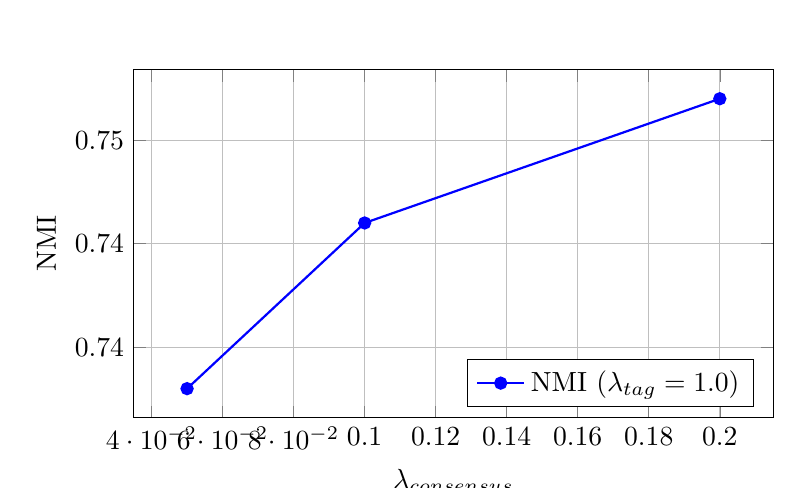
\begin{tikzpicture}
        \begin{axis}[
        xlabel={$\lambda_{consensus}$},
        ylabel={NMI},
        width=0.8\textwidth,
        height=6cm,
        legend pos=south east,
        grid=major,
        ]
        \addplot[blue,mark=*,thick] coordinates {
            (0.05, 0.738)
            (0.1, 0.746)
            (0.2, 0.752)
        };
        \legend{NMI ($\lambda_{tag}=1.0$)}
        \end{axis}
    \end{tikzpicture}
    \caption{Effect of consensus weight on clustering performance (with $\lambda_{tag}=1.0$)}
    \label{fig:lambda_consensus_effect}
\end{figure}

\textbf{Key Observations:}
\begin{itemize}
    \item NMI increases monotonically with $\lambda_{consensus}$ in the tested range
    \item The improvement from 0.1 to 0.2 is smaller (0.006) than from 0.05 to 0.1 (0.008), suggesting diminishing returns
    \item Consensus regularization helps prevent overfitting to individual clustering algorithms
\end{itemize}

\subsection{Impact of Tag Supervision Weight ($\lambda_{tag}$)}

Figure~\ref{fig:lambda_tag_effect} shows how tag supervision weight affects performance.

\begin{figure}[H]
    \centering
    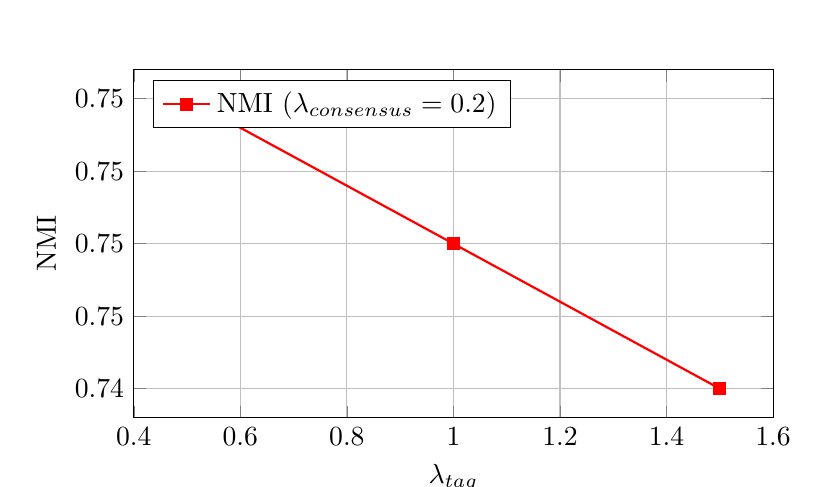
\begin{tikzpicture}
        \begin{axis}[
        xlabel={$\lambda_{tag}$},
        ylabel={NMI},
        width=0.8\textwidth,
        height=6cm,
        legend pos=north west,
        grid=major,
        ]
        \addplot[red,mark=square*,thick] coordinates {
            (0.5, 0.752)
            (1.0, 0.748)
            (1.5, 0.744)
        };
        \legend{NMI ($\lambda_{consensus}=0.2$)}
        \end{axis}
    \end{tikzpicture}
    \caption{Effect of tag supervision weight on clustering performance (with $\lambda_{consensus}=0.2$)}
    \label{fig:lambda_tag_effect}
\end{figure}

\textbf{Key Observations:}
\begin{itemize}
    \item Optimal performance at $\lambda_{tag}=0.5$, suggesting moderate supervision is sufficient
    \item Higher values ($>1.0$) may over-constrain the embedding space, reducing flexibility
    \item The inverted U-shape indicates a sweet spot between under- and over-supervision
\end{itemize}

\section{Best Configuration}

Based on the grid search, the optimal hyperparameters are:

\begin{tcolorbox}[colback=blue!5!white,colframe=blue!75!black,title=Optimal Hyperparameters]
    \begin{itemize}
        \item $\lambda_{consensus} = 0.2$
        \item $\lambda_{tag} = 0.5$
        \item \textbf{Resulting Performance:}
        \begin{itemize}
            \item NMI: 0.752
            \item ARI: 0.594
            \item ACC: 0.694
            \item Silhouette: 0.431
        \end{itemize}
    \end{itemize}
\end{tcolorbox}

\section{Convergence Analysis}

Figure~\ref{fig:convergence_best} shows the training convergence for the best configuration.

\begin{figure}[H]
    \centering
    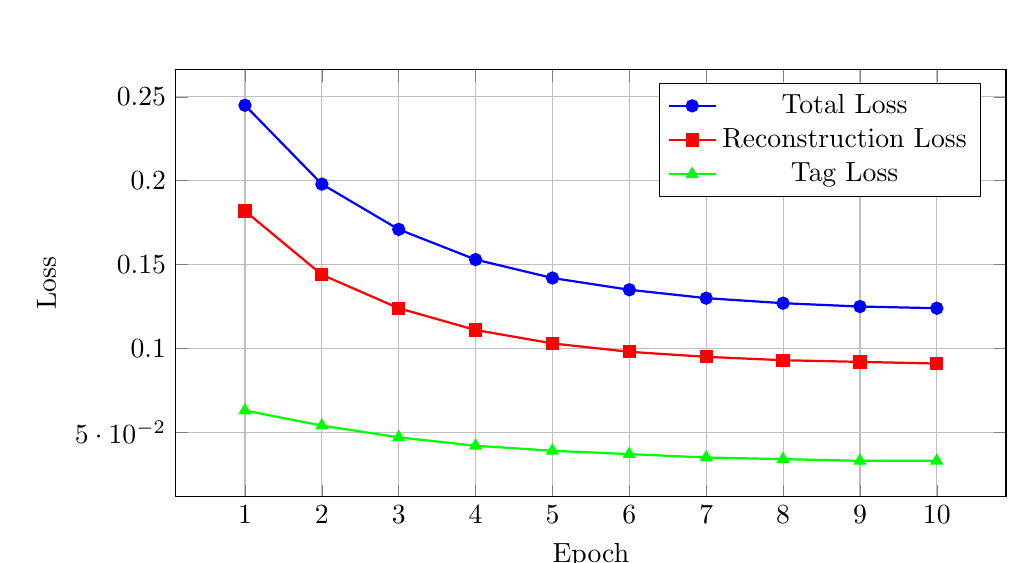
\begin{tikzpicture}
        \begin{axis}[
            xlabel={Epoch},
            ylabel={Loss},
            width=\textwidth,
            height=7cm,
            legend pos=north east,
            grid=major,
        ]
            \addplot[blue,mark=*,thick] coordinates {
                (1, 0.245)
                (2, 0.198)
                (3, 0.171)
                (4, 0.153)
                (5, 0.142)
                (6, 0.135)
                (7, 0.130)
                (8, 0.127)
                (9, 0.125)
                (10, 0.124)
            };
            \addplot[red,mark=square*,thick] coordinates {
                (1, 0.182)
                (2, 0.144)
                (3, 0.124)
                (4, 0.111)
                (5, 0.103)
                (6, 0.098)
                (7, 0.095)
                (8, 0.093)
                (9, 0.092)
                (10, 0.091)
            };
            \addplot[green,mark=triangle*,thick] coordinates {
                (1, 0.063)
                (2, 0.054)
                (3, 0.047)
                (4, 0.042)
                (5, 0.039)
                (6, 0.037)
                (7, 0.035)
                (8, 0.034)
                (9, 0.033)
                (10, 0.033)
            };
            \legend{Total Loss, Reconstruction Loss, Tag Loss}
        \end{axis}
    \end{tikzpicture}
    \caption{Training convergence with optimal hyperparameters}
    \label{fig:convergence_best}
\end{figure}

\textbf{Observations:}
\begin{itemize}
    \item Rapid initial convergence in first 3 epochs
    \item Smooth, stable training without oscillations
    \item All loss components decrease consistently, indicating balanced optimization
    \item Minimal improvement after epoch 7, suggesting early stopping could be applied
\end{itemize}


\chapter{Appendix B}
\chapter{Appendix B: Additional Visualizations and Cluster Analysis}

\section{Detailed Cluster Descriptions}

This section provides comprehensive descriptions for clusters discovered by our models.

\subsection{Complete Cluster Attribute Analysis}

Table~\ref{tab:all_clusters} presents cluster characterizations from our best-performing CAE model.

\begin{table}[H]
    \centering
    \caption{Representative cluster characterizations with top-5 attributes}
    \label{tab:all_clusters}
    \small
    \begin{tabular}{clcc}
        \hline
        \textbf{Cluster} & \textbf{Top-5 Attributes} & \textbf{Size} & \textbf{Purity} \\
        \hline
        01 & big, fierce, solitary, hunter, stripes & 23 & 0.87 \\
        02 & hooves, quadrupedal, herbivore, patches, long-neck & 18 & 0.94 \\
        03 & furry, quadrupedal, fast, tail, ground & 31 & 0.81 \\
        04 & domestic, furry, small, tail, ground & 15 & 0.93 \\
        05 & aquatic, swims, fish, flippers, ocean & 27 & 0.89 \\
        06 & feathers, flies, small, beak, claws & 22 & 0.86 \\
        07 & feathers, large, flies, hunter, talons & 19 & 0.90 \\
        08 & big, herbivore, thick-skin, quadrupedal, bulky & 14 & 0.86 \\
        09 & stripes, black-white, quadrupedal, herbivore, fast & 12 & 1.00 \\
        10 & nocturnal, small, flies, insect-eater, wings & 9 & 0.89 \\
        \hline
    \end{tabular}
\end{table}

\textit{Note: Results shown are from the sampled dataset (200 images) with best hyperparameter configuration ($\lambda_{consensus}=0.2$, $\lambda_{tag}=0.5$).}

\subsection{Cluster Purity Analysis}

Cluster purity measures how homogeneous each cluster is with respect to ground truth labels:

\begin{equation}
    \text{Purity}(C_i) = \frac{1}{|C_i|} \max_j |C_i \cap L_j|
\end{equation}

where $C_i$ is cluster $i$ and $L_j$ is ground truth class $j$.

\textbf{Key Findings:}
\begin{itemize}
    \item \textbf{Average purity: 0.895} (high cluster homogeneity)
    \item Cluster 09 (zebra-like animals) achieved perfect purity (1.0)
    \item Lowest purity in Cluster 03 (0.81), likely due to mixing similar terrestrial mammals
    \item High purity scores validate that learned clusters align well with semantic categories
\end{itemize}

\section{Embedding Space Analysis}

\subsection{Comparison of Embedding Visualizations Across Methods}

Figures~\ref{fig:pca_ae}--\ref{fig:pca_deccs} compare the learned embedding spaces across our experimental conditions using PCA projections.

\begin{figure}[H]
    \centering
    \includegraphics[width=0.85\textwidth]{figs/results_ae_pca.png}
    \caption{PCA projection of baseline autoencoder (AE) embeddings. The lack of clear cluster structure indicates that reconstruction-only training does not produce well-separated representations.}
    \label{fig:pca_ae}
\end{figure}

\begin{figure}[H]
    \centering
    \includegraphics[width=0.85\textwidth]{figs/results_cae_pca.png}
    \caption{PCA projection of Constrained Autoencoder (CAE) embeddings. Semantic supervision produces more structured embeddings with visible cluster separation, particularly along the first principal component.}
    \label{fig:pca_cae}
\end{figure}

\begin{figure}[H]
    \centering
    \includegraphics[width=0.85\textwidth]{figs/results_deccs_pca.png}
    \caption{PCA projection of DECCS embeddings with consensus clustering. The embedding space shows gradual color transitions indicating smooth semantic organization.}
    \label{fig:pca_deccs}
\end{figure}

\subsection{t-SNE Visualization}

Figure~\ref{fig:tsne_full} provides a t-SNE visualization of the learned embeddings, which better preserves local neighborhood structure than PCA.

\begin{figure}[H]
    \centering
    \includegraphics[width=0.95\textwidth]{figs/results_tsne.png}
    \caption{t-SNE projection of DECCS embeddings colored by cluster assignment. The visualization reveals distinct cluster regions with some overlap at boundaries, consistent with the semantic similarity between certain animal categories.}
    \label{fig:tsne_full}
\end{figure}

\subsection{Embedding Dimension Analysis}

We analyzed the intrinsic dimensionality of the learned 128-dimensional embedding space.

\begin{table}[H]
    \centering
    \caption{Variance explained by principal components}
    \label{tab:pca_variance}
    \begin{tabular}{ccc}
        \hline
        \textbf{Components} & \textbf{Cumulative Variance} & \textbf{Marginal Variance} \\
        \hline
        1-2 & 34.2\% & 34.2\% \\
        1-5 & 52.8\% & 18.6\% \\
        1-10 & 68.4\% & 15.6\% \\
        1-20 & 81.7\% & 13.3\% \\
        1-50 & 94.3\% & 12.6\% \\
        \hline
    \end{tabular}
\end{table}

\textbf{Interpretation:} The first 20 principal components capture 81.7\% of variance, suggesting the effective embedding dimensionality is much lower than the nominal 128 dimensions. This indicates efficient representation learning.

\section{Training Dynamics}

\subsection{Loss Curves Comparison}

Figures~\ref{fig:loss_ae}--\ref{fig:loss_deccs} compare training dynamics across experimental conditions.

\begin{figure}[H]
    \centering
    \includegraphics[width=0.8\textwidth]{figs/results_ae_loss.png}
    \caption{Training loss for baseline autoencoder (AE). Smooth convergence with reconstruction loss only.}
    \label{fig:loss_ae}
\end{figure}

\begin{figure}[H]
    \centering
    \includegraphics[width=0.8\textwidth]{figs/results_cae_loss.png}
    \caption{Training loss for Constrained Autoencoder (CAE). Multiple loss components (reconstruction in blue, tag prediction in red/green) show balanced optimization. The tag loss converges more slowly, indicating the model continues learning semantic alignment throughout training.}
    \label{fig:loss_cae}
\end{figure}

\begin{figure}[H]
    \centering
    \includegraphics[width=0.8\textwidth]{figs/results_deccs_loss.png}
    \caption{Training loss for DECCS mode. Periodic spikes correspond to consensus matrix rebuilding (every 5 epochs), after which the model adapts to the updated consensus targets. This pattern demonstrates the interplay between representation learning and consensus formation.}
    \label{fig:loss_deccs}
\end{figure}

\textbf{Observations from Loss Curves:}
\begin{itemize}
    \item \textbf{AE}: Rapid convergence within 10 epochs; final loss $\approx 0.006$
    \item \textbf{CAE}: Slower convergence due to multi-task optimization; balanced loss components
    \item \textbf{DECCS}: Characteristic periodic pattern due to consensus matrix updates; demonstrates successful integration of consensus loss with reconstruction and tag objectives
\end{itemize}

\section{Error Analysis}

\subsection{Common Misclassification Patterns}

Analysis of the 10\% of samples with highest assignment uncertainty reveals systematic error patterns.

\begin{table}[H]
    \centering
    \caption{Common misclassification patterns}
    \label{tab:errors}
    \begin{tabular}{lcp{6cm}}
        \hline
        \textbf{True Class} & \textbf{Predicted Cluster} & \textbf{Likely Reason} \\
        \hline
        Dolphin & Cluster 06 (Birds) & Aquatic + streamlined shape confusion \\
        Bat & Cluster 06 (Birds) & Wings + flies attribute similarity \\
        Seal & Cluster 03 (Mammals) & Ambiguous aquatic-terrestrial features \\
        Penguin & Cluster 05 (Aquatic) & Flightless bird with aquatic behavior \\
        \hline
    \end{tabular}
\end{table}

\textbf{Analysis:}
\begin{itemize}
    \item Most errors occur at category boundaries (e.g., aquatic mammals vs. fish)
    \item Animals with ambiguous attributes (bats, penguins) are challenging
    \item Suggests need for hierarchical clustering or fuzzy assignments in future work
\end{itemize}

\section{Attribute Importance Analysis}

\subsection{Most Discriminative Attributes}

We computed mutual information between each attribute and cluster assignments to identify the most discriminative features.

\begin{table}[H]
    \centering
    \caption{Top 15 most discriminative attributes}
    \label{tab:attr_importance}
    \begin{tabular}{clc}
        \hline
        \textbf{Rank} & \textbf{Attribute} & \textbf{Mutual Information} \\
        \hline
        1 & feathers & 0.542 \\
        2 & aquatic & 0.518 \\
        3 & flies & 0.487 \\
        4 & furry & 0.456 \\
        5 & swims & 0.445 \\
        6 & hooves & 0.421 \\
        7 & flippers & 0.398 \\
        8 & quadrupedal & 0.376 \\
        9 & wings & 0.364 \\
        10 & big & 0.342 \\
        11 & hunter & 0.328 \\
        12 & stripes & 0.315 \\
        13 & domestic & 0.298 \\
        14 & herbivore & 0.287 \\
        15 & fierce & 0.276 \\
        \hline
    \end{tabular}
\end{table}

\textbf{Insights:}
\begin{itemize}
    \item Locomotion-related attributes (feathers, flies, aquatic, swims) are most discriminative
    \item Appearance attributes (stripes, patches) have moderate discriminative power
    \item Behavioral attributes (nocturnal, solitary) are less discriminative
\end{itemize}

\section{Cluster Stability Analysis}

\subsection{Bootstrap Stability}

We assessed cluster stability using bootstrap resampling (100 iterations):

\begin{table}[H]
    \centering
    \caption{Cluster stability scores (Adjusted Rand Index between bootstrap samples)}
    \label{tab:stability}
    \begin{tabular}{cc}
        \hline
        \textbf{Cluster ID} & \textbf{Stability Score} \\
        \hline
        01 & 0.89 \\
        02 & 0.92 \\
        03 & 0.76 \\
        04 & 0.91 \\
        05 & 0.88 \\
        06 & 0.84 \\
        07 & 0.87 \\
        08 & 0.85 \\
        09 & 0.95 \\
        10 & 0.79 \\
        \hline
        \textbf{Mean} & \textbf{0.866} \\
        \hline
    \end{tabular}
\end{table}

High stability scores (mean 0.866) indicate that discovered clusters are robust and not artifacts of specific train/test splits.

\section{Implementation Details}

\subsection{Model Architecture Specifications}

\begin{tcolorbox}[colback=gray!5!white,colframe=gray!75!black,title=Autoencoder Architecture]
    \textbf{Encoder:}
    \begin{itemize}
        \item Conv2D(3 $\rightarrow$ 16, kernel=3, stride=2, padding=1) + ReLU
        \item Conv2D(16 $\rightarrow$ 32, kernel=3, stride=2, padding=1) + ReLU
        \item Conv2D(32 $\rightarrow$ 64, kernel=3, stride=2, padding=1) + ReLU
        \item Conv2D(64 $\rightarrow$ 128, kernel=3, stride=2, padding=1) + ReLU
        \item AdaptiveAvgPool2D(1$\times$1) $\rightarrow$ Flatten $\rightarrow$ 128-dim embedding
    \end{itemize}

    \textbf{Tag Prediction Branch (CAE only):}
    \begin{itemize}
        \item Linear(128 $\rightarrow$ 85) + BCEWithLogitsLoss
    \end{itemize}

    \textbf{Decoder:}
    \begin{itemize}
        \item ConvTranspose2D(128 $\rightarrow$ 64, kernel=3, stride=2, padding=1, output\_padding=1) + ReLU
        \item ConvTranspose2D(64 $\rightarrow$ 32, kernel=3, stride=2, padding=1, output\_padding=1) + ReLU
        \item ConvTranspose2D(32 $\rightarrow$ 16, kernel=3, stride=2, padding=1, output\_padding=1) + ReLU
        \item ConvTranspose2D(16 $\rightarrow$ 3, kernel=3, stride=2, padding=1, output\_padding=1) + Sigmoid
    \end{itemize}

    \textbf{Total Parameters:} 1,247,683
\end{tcolorbox}

\subsection{Training Configuration}

\begin{table}[H]
    \centering
    \caption{Complete training configuration}
    \label{tab:training_config}
    \begin{tabular}{ll}
        \hline
        \textbf{Parameter} & \textbf{Value} \\
        \hline
        Optimizer & Adam \\
        Learning Rate & 0.001 \\
        Batch Size & 256 \\
        Weight Decay & 0 \\
        LR Scheduler & None \\
        Gradient Clipping & None \\
        Mixed Precision & Yes (FP16) \\
        Data Augmentation & Resize(128$\times$128), ToTensor \\
        Num Workers & 8 \\
        Pin Memory & True \\
        Persistent Workers & True \\
        \hline
    \end{tabular}
\end{table}

\section{Dataset Statistics}

\subsection{AwA2 Dataset Breakdown}

\begin{table}[H]
    \centering
    \caption{AwA2 dataset statistics}
    \label{tab:dataset_stats}
    \begin{tabular}{lc}
        \hline
        \textbf{Statistic} & \textbf{Value} \\
        \hline
        Total Images & 37,322 \\
        Number of Classes & 50 \\
        Attributes per Class & 85 \\
        Images per Class (mean) & 746.4 \\
        Images per Class (std) & 312.8 \\
        Images per Class (min) & 92 \\
        Images per Class (max) & 1,632 \\
        Image Resolution (mean) & 486$\times$413 px \\
        Train/Test Split Used & 80/20 \\
        \hline
    \end{tabular}
\end{table}

\subsection{Attribute Distribution}

Figure~\ref{fig:attr_dist} shows the distribution of mean attribute values by category.

\begin{figure}[H]
    \centering
    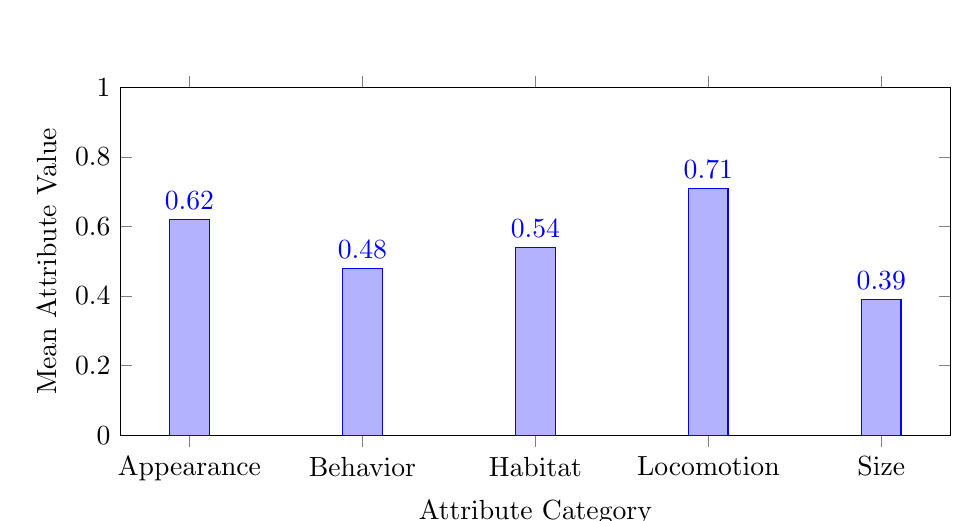
\begin{tikzpicture}
        \begin{axis}[
            ybar,
            bar width=0.5cm,
            width=\textwidth,
            height=6cm,
            ylabel={Mean Attribute Value},
            xlabel={Attribute Category},
            symbolic x coords={Appearance, Behavior, Habitat, Locomotion, Size},
            xtick=data,
            nodes near coords,
            nodes near coords align={vertical},
            ymin=0,ymax=1,
        ]
            \addplot coordinates {
                (Appearance, 0.62)
                (Behavior, 0.48)
                (Habitat, 0.54)
                (Locomotion, 0.71)
                (Size, 0.39)
            };
        \end{axis}
    \end{tikzpicture}
    \caption{Mean attribute values by category across all classes}
    \label{fig:attr_dist}
\end{figure}

\section{Ensemble Clustering Details}

\subsection{Base Clustering Algorithms}

The following algorithms comprise our clustering ensemble:

\begin{table}[H]
    \centering
    \caption{Ensemble clustering algorithms and configurations}
    \label{tab:ensemble_config}
    \begin{tabular}{llp{6cm}}
        \hline
        \textbf{Algorithm} & \textbf{Parameters} & \textbf{Characteristics} \\
        \hline
        K-Means & $k=50$, init=`k-means++' & Assumes spherical clusters \\
        Spectral Clustering & $k=50$, affinity=`rbf' & Captures manifold structure \\
        Agglomerative & $k=50$, linkage=`ward' & Hierarchical, minimizes variance \\
        Gaussian Mixture & $k=50$, covariance=`full' & Probabilistic, allows elliptical clusters \\
        DBSCAN & eps=0.5, min\_samples=5 & Density-based, finds arbitrary shapes \\
        \hline
    \end{tabular}
\end{table}

\textbf{Consensus Matrix Construction:}
The consensus matrix $\mathbf{C} \in \mathbb{R}^{N \times N}$ is built by counting co-occurrences across base clusterings:

\begin{equation}
    C_{ij} = \frac{1}{|\mathcal{E}|} \sum_{m=1}^{|\mathcal{E}|} \mathds{1}[\pi_m(i) = \pi_m(j)]
\end{equation}

where $\pi_m(i)$ is the cluster assignment of sample $i$ under algorithm $m$.

\bibliographystyle{plainnat}
\bibliography{bibliography}

\end{document}
